\begin{CJK}{Bg5}{bsmi}

%---------------------------------------------
%	Chapter System Architecture
%---------------------------------------------

\chapter{System Architecture}

In this chapter, I'll try to explain my design more detailed. First section is the basic idea of my authentication system, which is based on digital signature algorithm. The next section is about the flow if clinets and servers adopt this scheme. The next chapter gives two demonstrations of this scheme. One is for the furture website, and one if for the existing website. The last section gives a high-level code example to explain how to implement this system.

\section{Overview}

Let us recall the autehentication process about password-based scheme. As the fig\ref{fig:password-based-flow} shows, the client give his username and password to server (password is encrypted), and the server checks whether it is valid according to its database. Fig\ref{fig:my-scheme-flow} is the authentication process of my scheme. Because the verificaiton server should be a passive element, client should send a login request first. After receive a login request, the server send a random nonce back to client. Client generate a signature for this nonce and return to server. Server, then, use the public key to check whether the client is valid or not.

\begin{figure}
\centering
\subfigure[password-based scheme]{
\label{fig:password-based-flow}
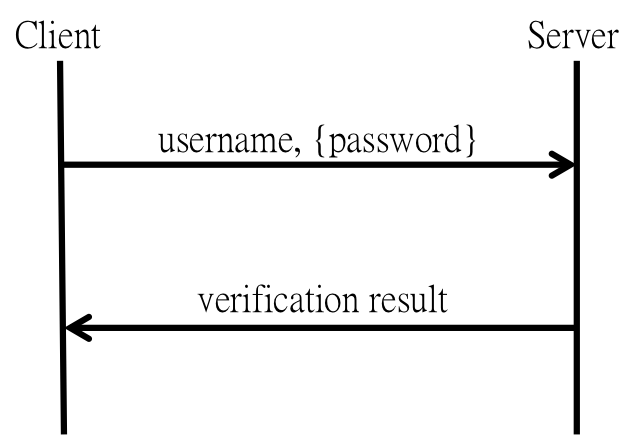
\includegraphics[scale=0.6]{picture/password-based-flow.png}
}
\subfigure[my scheme]{
\label{fig:my-scheme-flow}
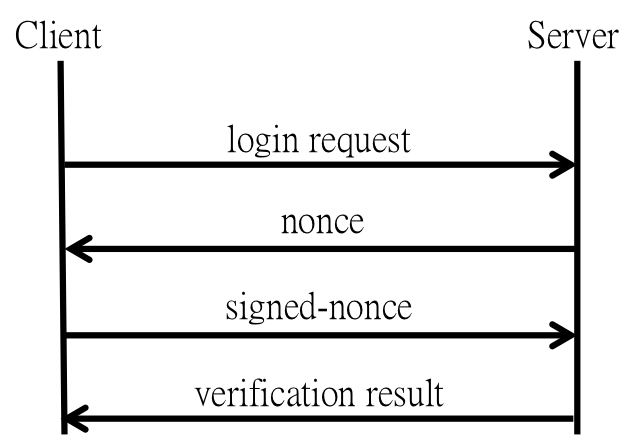
\includegraphics[scale=0.6]{picture/basic-idea-flow.png}
}
\caption{Authentication flow}
\end{figure}

This is how I used Digital Signature Algorithms in an authentication process. The advantages is that the data communicated between client and server do not need to be encrypted. The only \emph{secret} is private key, which is stored in client's storage. The disavantage of my scheme is that users will need a device to help them creating signature and manage their public keys. Therefore, the use of mobile device is the core of this scheme, bring us a high usability. The user flow become fig\ref{final-flow} with the help of mobile device.

\begin{figure}
\centering
\label{fig:final-flow}
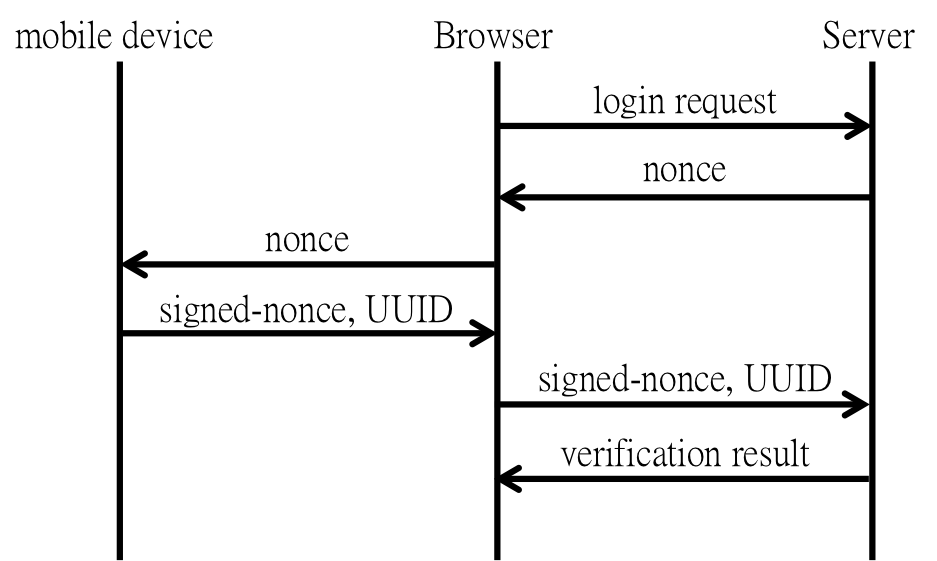
\includegraphics[scale=0.65]{picture/final-flow.png}
\caption{Authentication flow with mobile device}
\end{figure}

\section{User Flow}

In this section, I'll seperate the autentication process into three parts: \emph{register phase}, \emph{login phase} and \emph{verification phase}.

\subsubsection{Register Phase}

	1. 	User start the initialzization process on his mobile device
		i.  set PIN code
		ii. generate key pair
	2.	User send a registration request to server from browser

	3.	User send his id and public key (and other required credentials) to server.

\subsubsection{Login Phase}

	1. User send a login requesr to server

	2. Server return a nonce ({server info || randombits}) back to browser

	3. The brower pass this nonce to reader application
		i.	The reader start to scan NFC cards.
		ii.	Timeout: 30 seconds

	4. Mobile device ask user to input the correct PIN code and confirm the server information
		i.	Enable card emulation mode right after receive correct PIN code

	5. Mobile device get nonce from reader application
		i.	mobile device signed the nonce with correspond private key.
		ii.	mobile device return the signed-nonce back to reader application

	6. Reader application return signed-nonce back to server.

\subsubsection{Verification Phase}

	1. Server find the corresponding public key accordding to id.

	2. Verify the signature.

	3. Return the result.

\section{Scenario}

\subsection{Future Website}

\subsection{Existing Website}

\section{Implementation}

\end{CJK}